\documentclass[]{article} % for elsevier submission
\usepackage{amsmath}
\usepackage{graphicx,psfrag,epsf}
\usepackage{enumerate}
\usepackage{natbib}
\usepackage{textcomp}
\usepackage[hyphens]{url} % not crucial - just used below for the URL
\usepackage{hyperref}
\usepackage{listings} 
\usepackage{booktabs}
\usepackage{float}
\usepackage{threeparttable}
\usepackage{threeparttablex}
%\usepackage[onehalfspacing]{setspace}
\usepackage{ebgaramond}
\usepackage[varqu,varl,var0,scaled=0.97]{inconsolata} 
\usepackage{FiraSans}
\usepackage[usenames,dvipsnames]{color}    
\usepackage[font=small, font+=singlespacing,labelfont=bf]{caption}
%\usepackage[pagewise]{lineno}
\PassOptionsToPackage{usenames,dvipsnames,svgnames}{xcolor}  
\usepackage{tikz}
\usetikzlibrary{arrows,positioning,automata}

\title{Mediation}
\author{Stijn Masschelein}
\date{April 2020}

\begin{document}

\maketitle

\section{Mediation Analysis}
\subsection{Simple Mediation in Experiment}

\begin{tikzpicture}[>=stealth',shorten >=1pt,node distance=3cm,on grid,initial/.style    ={}]
  \node[state]          (M)                  {$M$};
  \node[state]          (X) [left =of M]    {$X$};
  \node[state]          (Y) [right =of M]    {$Y$};
  \node[state]          (W) [above right =of M]    {$W$};
  \node[state]          (V) [below =of M]    {$V$};
\tikzset{mystyle/.style={->}}   
\path (X)     edge [mystyle] (M)
      (M)     edge [mystyle] (Y) 
      (W)     edge [mystyle] (M)
      (W)     edge [mystyle] (Y)
      (X)     edge [mystyle] (V)
      (V)     edge [mystyle] (Y);
\end{tikzpicture}

\begin{figure}    
\centering
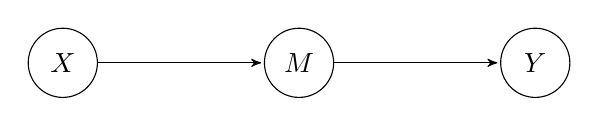
\begin{tikzpicture}[>=stealth',shorten >=1pt,node distance=3cm,on grid,initial/.style    ={}]
  \node[state]          (M)                  {$M$};
  \node[state]          (X) [left =of M]    {$X$};
  \node[state]          (Y) [right =of M]    {$Y$};
\tikzset{mystyle/.style={->}}
\path (X)     edge [mystyle] (M)
      (M)     edge [mystyle] (Y);
\end{tikzpicture}
\caption{The basic moderation DAG} \label{basic}
\end{figure}


$X$ is manipulated in an experiment. $M$ is the mediator. $Y$ is the outcome of interest. 

$W$ is a confounding factor. If $W$ exists, you need to use an instrumental variable approach to get an unbiased estimate of $M -> Y$. The instrumental variable approach is only valid if there is no $V$.

Interestingly enough if there is an observed $W == V$ both approaches are doomed if you do not measure the $W == V$ variable.

\subsection{TODO}
\begin{enumerate}
    \item Look up Rosenbaum's gamma as a way to test the sensitivity to bias from confounders.
    \item Are we looking at statistical problems or bias. The simulation paper started from bias but the simulations showed the problem with inference (s.e. were wrong).
\end{enumerate}
\section{Second Order Factor Complementarity}
\subsection{From the review}

There are two problems with this approach. First, the common factor
approach cannot distinguish between the three-way effect and the
effect of the three two-way effects. Second, it's not a necessary
condition for a three-way effect to exist for three practices to form
a system.

One way of seeing the problem with the common factor approach is the
following numerical example. Let's assume that two combinations of two
practices are complements. For instance practice 1 and 2, and practice
1 and 3 are complements. That implies that in equilibrium, the
conditional correlation between 1 and 2 (cor12) and between 1 and 3
(cor13) will be positive. Let's say cor12 = 0.6, and cor13 = 0.6, in
the absence of any complementarity between 2 and 3, the conditional
correlation cor23 = cor12 x cor13 = 0.36. We cannot perform a factor
analysis with this information but we can calculate the Cronbach's
alpha as a measure of internal consistency which equals k x r / (1 +
(k - 1) x r) where k is the number of correlations and r is the
average correlation. In the example, the Cronbach's alpha is equal to
0.76 which would indicate internal consistency. 

Another way of looking at this is that if for whatever reason the cost
of practice 2 increases, the unit will also decrease the use of
practice 1 (the first complementarity) and because 1 decreases,
practice 3 will also decrease (the second complementarity). That is
practice 3 depends on practice 2 through practice 1 and the three
practices form a system in the absence of any three-way
interdependency.

For instance, take two identical units A and B in the example with two
complementarities from above. If the cost of practice 2 increases for
unit A, the optimal behavior for A is to decrease the use of the three
practices. If the cost of practice 2 decreases for unit B, the optimal
behavior for B is to increase the use of the three practices. A and B
both have the optimal system but they have different levels of
use. The common factor will pick up the fact that the level for the
three practices moves together (all up for A, all down for B). 
However, if there is a difference in effectiveness between A and B
it's not because of the use of the practices (they are both optimal), 
it's because the cost of practice 2 is higher for A than it is for B. 

The correct approach would be to try to identify the deviation from
the optimal approach. For instance take a unit C, where the cost of
practice 2 decreases, but they only increase the use of practice 2 and
not the other practices.  Now, unit C has not chosen the optimal
level and we would expect that level C has a lower effectiveness than
B. This example shows that it's not important to measure which of the
many possible optimal systems the unit is using (i.e. the factor
score) but whether they deviate from the optimal level for their
circumstances. 
 
The correct way to use the common factor approach is to use the
deviations from the optimal common factor, i.e. the error terms es1,
es2, and es3 in Figure 2. If the absolute deviation of the optimal
level is higher, we should see lower effectiveness. I am personally
sceptical about this approach in practice. It assumes that the units
are on average in equilibrium but with still enough variation left to
detect performance differences. This likely means that both the common
factor approach is misspecified (units are not on average in
equilibrium) and the deviations approach is misspecified because it
assumes that the common factor approach works to identify the optimal
levels. In addition, the deviations approach will also lack power if
most units are close to the optimal level. In my opinion, it's not
necessary to use the deviation approach because it's unlikely to yield
significant results because of the lack of power and might lead to
false positives because of the misspecification issue. 

\subsection{References}

\begin{enumerate}
    \item Patient zero: https://doi-org.ezproxy.library.uwa.edu.au/10.1002/smj.435
    \item The meta analysis: https://doi-org.ezproxy.library.uwa.edu.au/10.1002/smj.3042
\end{enumerate}

\subsection{Structure of a paper: Complementaries, common factors, and indices: Righting some wrongs}

\subsubsection{Theory}

$\vec{x}$ is the $N$ choices and $\vec{z}$ is the $M$ environmental factors determining the costs and benefits of the choices. $y$ is the performance of the firm. $\vec{\beta}$ are the direct performance effects of the choices when $\vec{z} = \vec{0}$. $\vec{\delta}$ are the 
$G$ is a $M \times N$ matrix and determines the cost and benefits based on the environmental factors. $B$ is an $N$-square matrix with $0$ diagonal and captures the complementarities between the choices. Let $A = \delta^T I_N - B$. 

The production function is then the following equation.
\begin{equation}
\label{eq:production}
    y = (\vec{\beta}^T + \vec{z}^T G + \vec{\epsilon}^T) \vec{x} 
         - \frac{1}{2} \vec{x}^T A \vec{x} + \nu
\end{equation}

The optimal choices are given by 
\begin{equation}
\label{eq:optimal}
    \vec{x^*} = A^{-1}(\vec{\beta}^T + \vec{z}^T G + \vec{\epsilon}^T) 
\end{equation}

as long as $A$ is negative definite.

https://www.tulane.edu/~PsycStat/dunlap/Psyc613/RI2.html. This source makes the link between the determinant of scaled A and how much the 

\subsubsection{Covariance Structure}
From \ref{eq:optimal}, it's relatively easy to derive the covariance matrix
$X^*{X^{*}}^T$ for a sample of optimal decisions. It' easy to see that the covariance depends on $Z$ as well as $A$, thus the need to control for the environment when testing 
for complementarities.

After centering of $Z$ and assuming $Z E = 0$

\begin{align}
\Sigma_x = X^TX 
     &= ((Z G + E)A^{-1})^T (Z G + E)A^{-1} \nonumber \\
     &= A^{-1} (G^T Z^T + E^T) (G Z + E) A^{-1} \nonumber \\
     &= A^{-1} (G^T \Sigma_z G + \Sigma_{\epsilon}) A^{-1} \label{eq:covariance}
\end{align}

This also means that both complementarity and the environment can be underlying reasons for the covariance. 

\subsubsection{One factor model}

See also VanderWeele for one factor model, $\eta$.

\begin{align*}
    \vec{x} &= \vec{\lambda} \eta + \vec{\delta} \\
    \vec{x} - \vec{\delta} &= \vec{\lambda} \eta \\
    \vec{\lambda}^{-1} (\vec{x} - \vec{\delta}) &= \eta \\ 
    \sum \frac{x_i - \delta_i}{\lambda_i} &= \eta \\
\end{align*}

See Bollen (1989) in Chapter 4 on identification to find closed form solutions for a 
one factor model.

The model has $2n + 1$ parameters. The covariance has $\frac{n (n+1)}{2}$ pieces of information. Assuming independence of errors.

\begin{align*}
    \vec{x} &= \vec{\lambda} \eta + \vec{\delta} \\
    E(\vec{x} \vec{x}^{T}) &= (\vec{\lambda} \eta + \vec{\delta})
        (\vec{\lambda} \eta + \vec{\delta})^{T} \\
    &= \sigma_{\eta} \vec{\lambda} \vec{\lambda}^{T} + \vec{\sigma_{\delta}} I_n \\
    E(x_i x_j) &= \sigma_{\eta} \lambda_i \lambda_j \\ 
    E(x_i x_i) &= \sigma_{\eta} \lambda_i^2 + {\sigma_{\delta}}_{ii}
\end{align*}

\subsubsection{Goldilock}

The Goldilock zone of just close enough to identify the weights but not enough to completely wash out the performance effects.

\subsubsection{An index}

Literature ignoring the issue that firm's make choices. Voluntary disclosure.

An index with weights, $\vec{w}$. This is a more general form of the common factor model.

\begin{equation}
\label{eq:index}
    \Sigma w_i x^*_i = 
    \Sigma w_i [[A^{-1}]_i (\vec{\beta}^T + \vec{z}^T G + \vec{\epsilon}^T)]
\end{equation}


\end{document}